% Options for packages loaded elsewhere
\PassOptionsToPackage{unicode}{hyperref}
\PassOptionsToPackage{hyphens}{url}
%
\documentclass[
]{book}
\usepackage{amsmath,amssymb}
\usepackage{lmodern}
\usepackage{iftex}
\ifPDFTeX
  \usepackage[T1]{fontenc}
  \usepackage[utf8]{inputenc}
  \usepackage{textcomp} % provide euro and other symbols
\else % if luatex or xetex
  \usepackage{unicode-math}
  \defaultfontfeatures{Scale=MatchLowercase}
  \defaultfontfeatures[\rmfamily]{Ligatures=TeX,Scale=1}
\fi
% Use upquote if available, for straight quotes in verbatim environments
\IfFileExists{upquote.sty}{\usepackage{upquote}}{}
\IfFileExists{microtype.sty}{% use microtype if available
  \usepackage[]{microtype}
  \UseMicrotypeSet[protrusion]{basicmath} % disable protrusion for tt fonts
}{}
\makeatletter
\@ifundefined{KOMAClassName}{% if non-KOMA class
  \IfFileExists{parskip.sty}{%
    \usepackage{parskip}
  }{% else
    \setlength{\parindent}{0pt}
    \setlength{\parskip}{6pt plus 2pt minus 1pt}}
}{% if KOMA class
  \KOMAoptions{parskip=half}}
\makeatother
\usepackage{xcolor}
\IfFileExists{xurl.sty}{\usepackage{xurl}}{} % add URL line breaks if available
\IfFileExists{bookmark.sty}{\usepackage{bookmark}}{\usepackage{hyperref}}
\hypersetup{
  pdftitle={R과 통계분석},
  pdfauthor={박동련},
  hidelinks,
  pdfcreator={LaTeX via pandoc}}
\urlstyle{same} % disable monospaced font for URLs
\usepackage{longtable,booktabs,array}
\usepackage{calc} % for calculating minipage widths
% Correct order of tables after \paragraph or \subparagraph
\usepackage{etoolbox}
\makeatletter
\patchcmd\longtable{\par}{\if@noskipsec\mbox{}\fi\par}{}{}
\makeatother
% Allow footnotes in longtable head/foot
\IfFileExists{footnotehyper.sty}{\usepackage{footnotehyper}}{\usepackage{footnote}}
\makesavenoteenv{longtable}
\usepackage{graphicx}
\makeatletter
\def\maxwidth{\ifdim\Gin@nat@width>\linewidth\linewidth\else\Gin@nat@width\fi}
\def\maxheight{\ifdim\Gin@nat@height>\textheight\textheight\else\Gin@nat@height\fi}
\makeatother
% Scale images if necessary, so that they will not overflow the page
% margins by default, and it is still possible to overwrite the defaults
% using explicit options in \includegraphics[width, height, ...]{}
\setkeys{Gin}{width=\maxwidth,height=\maxheight,keepaspectratio}
% Set default figure placement to htbp
\makeatletter
\def\fps@figure{htbp}
\makeatother
\setlength{\emergencystretch}{3em} % prevent overfull lines
\providecommand{\tightlist}{%
  \setlength{\itemsep}{0pt}\setlength{\parskip}{0pt}}
\setcounter{secnumdepth}{5}
\usepackage{booktabs}
\ifLuaTeX
  \usepackage{selnolig}  % disable illegal ligatures
\fi
\usepackage[]{natbib}
\bibliographystyle{plainnat}

\title{R과 통계분석}
\author{박동련}
\date{2022-07-06}

\begin{document}
\maketitle

{
\setcounter{tocdepth}{1}
\tableofcontents
}
\hypertarget{uxc18cuxac1cuxd558uxae30}{%
\chapter*{소개하기}\label{uxc18cuxac1cuxd558uxae30}}
\addcontentsline{toc}{chapter}{소개하기}

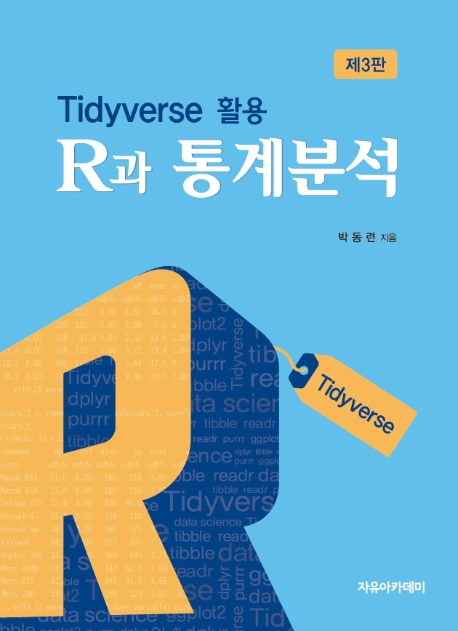
\includegraphics{Figure/cover.jpg}

\hypertarget{r-uxc2dcuxc791uxd558uxae30}{%
\chapter{R 시작하기}\label{r-uxc2dcuxc791uxd558uxae30}}

Placeholder

\hypertarget{ruxc758-uxc18cuxac1c}{%
\section{R의 소개}\label{ruxc758-uxc18cuxac1c}}

\hypertarget{ruxc758-uxc124uxce58}{%
\section{R의 설치}\label{ruxc758-uxc124uxce58}}

\hypertarget{rstudiouxc758-uxc124uxce58-uxbc0f-ruxc758-uxc2e4uxd589}{%
\section{RStudio의 설치 및 R의 실행}\label{rstudiouxc758-uxc124uxce58-uxbc0f-ruxc758-uxc2e4uxd589}}

\hypertarget{uxc791uxc5c5uxacf5uxac04}{%
\section{작업공간}\label{uxc791uxc5c5uxacf5uxac04}}

\hypertarget{uxc2a4uxd06cuxb9bduxd2b8-uxd30cuxc77cuxc758-uxd65cuxc6a9}{%
\section{스크립트 파일의 활용}\label{uxc2a4uxd06cuxb9bduxd2b8-uxd30cuxc77cuxc758-uxd65cuxc6a9}}

\hypertarget{section-batch}{%
\section{일괄처리}\label{section-batch}}

\hypertarget{section-package}{%
\section{R의 확장: 패키지}\label{section-package}}

\hypertarget{uxd328uxd0a4uxc9c0uxc758-uxc885uxb958}{%
\subsection{패키지의 종류}\label{uxd328uxd0a4uxc9c0uxc758-uxc885uxb958}}

\hypertarget{uxd328uxd0a4uxc9c0uxc758-uxc124uxce58-uxbc0f-uxc0acuxc6a9}{%
\subsection{패키지의 설치 및 사용}\label{uxd328uxd0a4uxc9c0uxc758-uxc124uxce58-uxbc0f-uxc0acuxc6a9}}

\hypertarget{uxd328uxd0a4uxc9c0-tidyverseuxc758-uxc18cuxac1c}{%
\subsection{\texorpdfstring{패키지 \texttt{tidyverse}의 소개}{패키지 tidyverse의 소개}}\label{uxd328uxd0a4uxc9c0-tidyverseuxc758-uxc18cuxac1c}}

\hypertarget{data-structure}{%
\chapter{R 데이터 구조}\label{data-structure}}

Placeholder

\hypertarget{uxbca1uxd130}{%
\section{벡터}\label{uxbca1uxd130}}

\hypertarget{uxbca1uxd130uxc758-uxae30uxbcf8-uxd2b9uxc131}{%
\subsection{벡터의 기본 특성}\label{uxbca1uxd130uxc758-uxae30uxbcf8-uxd2b9uxc131}}

\hypertarget{uxb2e4uxc591uxd55c-uxd615uxd0dcuxb97c-uxac16uxb294-uxbca1uxd130uxc758-uxc0dduxc131}{%
\subsection{다양한 형태를 갖는 벡터의 생성}\label{uxb2e4uxc591uxd55c-uxd615uxd0dcuxb97c-uxac16uxb294-uxbca1uxd130uxc758-uxc0dduxc131}}

\hypertarget{uxbca1uxd130uxc5d0-uxb370uxc774uxd130-uxcd94uxac00-uxbc0f-uxbca1uxd130uxb4e4uxc758-uxacb0uxd569}{%
\subsubsection{벡터에 데이터 추가 및 벡터들의 결합}\label{uxbca1uxd130uxc5d0-uxb370uxc774uxd130-uxcd94uxac00-uxbc0f-uxbca1uxd130uxb4e4uxc758-uxacb0uxd569}}

\hypertarget{uxc77cuxc815uxd55c-uxad6cuxc870uxb97c-uxac16uxb294-uxbca1uxd130uxc758-uxc0dduxc131}{%
\subsubsection{일정한 구조를 갖는 벡터의 생성}\label{uxc77cuxc815uxd55c-uxad6cuxc870uxb97c-uxac16uxb294-uxbca1uxd130uxc758-uxc0dduxc131}}

\hypertarget{uxbb38uxc790uxc5f4uxc744-uxc704uxd55c-uxd568uxc218}{%
\subsection{문자열을 위한 함수}\label{uxbb38uxc790uxc5f4uxc744-uxc704uxd55c-uxd568uxc218}}

\hypertarget{uxbca1uxd130uxc758-uxc5f0uxc0b0}{%
\subsection{벡터의 연산}\label{uxbca1uxd130uxc758-uxc5f0uxc0b0}}

\hypertarget{vector-compare}{%
\subsection{벡터의 비교}\label{vector-compare}}

\hypertarget{uxbca1uxd130uxc758-uxc778uxb371uxc2f1}{%
\subsection{벡터의 인덱싱}\label{uxbca1uxd130uxc758-uxc778uxb371uxc2f1}}

\hypertarget{uxc694uxc778}{%
\section{요인}\label{uxc694uxc778}}

\hypertarget{uxc694uxc778uxc758-uxae30uxbcf8-uxd2b9uxc131}{%
\subsection{요인의 기본 특성}\label{uxc694uxc778uxc758-uxae30uxbcf8-uxd2b9uxc131}}

\hypertarget{uxc22buxc790uxd615-uxbca1uxd130uxb97c-uxc694uxc778uxc73cuxb85c-uxbcc0uxd658}{%
\subsection{숫자형 벡터를 요인으로 변환}\label{uxc22buxc790uxd615-uxbca1uxd130uxb97c-uxc694uxc778uxc73cuxb85c-uxbcc0uxd658}}

\hypertarget{uxb0a0uxc9dc}{%
\section{날짜}\label{uxb0a0uxc9dc}}

\hypertarget{uxd589uxb82c-uxbc0f-uxbc30uxc5f4}{%
\section{행렬 및 배열}\label{uxd589uxb82c-uxbc0f-uxbc30uxc5f4}}

\hypertarget{uxd589uxb82cuxacfc-uxbc30uxc5f4uxc758-uxae30uxbcf8-uxd2b9uxc131}{%
\subsection{행렬과 배열의 기본 특성}\label{uxd589uxb82cuxacfc-uxbc30uxc5f4uxc758-uxae30uxbcf8-uxd2b9uxc131}}

\hypertarget{uxd589uxb82cuxc758-uxc5f0uxc0b0}{%
\subsection{행렬의 연산}\label{uxd589uxb82cuxc758-uxc5f0uxc0b0}}

\hypertarget{section-dataframe}{%
\section{데이터 프레임}\label{section-dataframe}}

\hypertarget{uxb370uxc774uxd130-uxd504uxb808uxc784uxc758-uxc0dduxc131}{%
\subsection{데이터 프레임의 생성}\label{uxb370uxc774uxd130-uxd504uxb808uxc784uxc758-uxc0dduxc131}}

\hypertarget{uxb370uxc774uxd130-uxd504uxb808uxc784uxc758-uxc778uxb371uxc2f1}{%
\subsection{데이터 프레임의 인덱싱}\label{uxb370uxc774uxd130-uxd504uxb808uxc784uxc758-uxc778uxb371uxc2f1}}

\hypertarget{uxd568uxc218-with}{%
\subsection{\texorpdfstring{함수 \texttt{with()}}{함수 with()}}\label{uxd568uxc218-with}}

\hypertarget{tibble-uxac1cuxc120uxb41c-uxd615uxd0dcuxc758-uxb370uxc774uxd130-uxd504uxb808uxc784}{%
\section{Tibble: 개선된 형태의 데이터 프레임}\label{tibble-uxac1cuxc120uxb41c-uxd615uxd0dcuxc758-uxb370uxc774uxd130-uxd504uxb808uxc784}}

\hypertarget{tibble-uxc0dduxc131}{%
\subsection{Tibble 생성}\label{tibble-uxc0dduxc131}}

\hypertarget{tibbleuxacfc-uxc804uxd1b5uxc801uxc778-uxb370uxc774uxd130-uxd504uxb808uxc784uxc758-uxcc28uxc774}{%
\subsection{Tibble과 전통적인 데이터 프레임의 차이}\label{tibbleuxacfc-uxc804uxd1b5uxc801uxc778-uxb370uxc774uxd130-uxd504uxb808uxc784uxc758-uxcc28uxc774}}

\hypertarget{section-list}{%
\section{리스트}\label{section-list}}

\hypertarget{uxc5f0uxc2b5uxbb38uxc81c}{%
\section{연습문제}\label{uxc5f0uxc2b5uxbb38uxc81c}}

\hypertarget{uxb370uxc774uxd130-uxc785uxb825}{%
\chapter{데이터 입력}\label{uxb370uxc774uxd130-uxc785uxb825}}

Placeholder

\hypertarget{uxd14duxc2a4uxd2b8-uxd30cuxc77c-uxbd88uxb7ecuxc624uxae30-uxd328uxd0a4uxc9c0-readr-uxd568uxc218uxc758-uxd65cuxc6a9}{%
\section{\texorpdfstring{텍스트 파일 불러오기: 패키지 \texttt{readr} 함수의 활용}{텍스트 파일 불러오기: 패키지 readr 함수의 활용}}\label{uxd14duxc2a4uxd2b8-uxd30cuxc77c-uxbd88uxb7ecuxc624uxae30-uxd328uxd0a4uxc9c0-readr-uxd568uxc218uxc758-uxd65cuxc6a9}}

\hypertarget{uxd568uxc218-read_tableuxb85c-uxb370uxc774uxd130-uxd30cuxc77c-uxbd88uxb7ecuxc624uxae30}{%
\subsection{\texorpdfstring{함수 \texttt{read\_table()}로 데이터 파일 불러오기}{함수 read\_table()로 데이터 파일 불러오기}}\label{uxd568uxc218-read_tableuxb85c-uxb370uxc774uxd130-uxd30cuxc77c-uxbd88uxb7ecuxc624uxae30}}

\hypertarget{uxd568uxc218-read_csvuxb85c-csv-uxb370uxc774uxd130-uxd30cuxc77c-uxbd88uxb7ecuxc624uxae30}{%
\subsection{\texorpdfstring{함수 \texttt{read\_csv()}로 CSV 데이터 파일 불러오기}{함수 read\_csv()로 CSV 데이터 파일 불러오기}}\label{uxd568uxc218-read_csvuxb85c-csv-uxb370uxc774uxd130-uxd30cuxc77c-uxbd88uxb7ecuxc624uxae30}}

\hypertarget{uxd568uxc218-read_fwfuxb85c-uxace0uxc815-uxd3ecuxb9f7-uxad6cuxc870uxb97c-uxac16uxb294-uxb370uxc774uxd130-uxd30cuxc77c-uxbd88uxb7ecuxc624uxae30}{%
\subsection{\texorpdfstring{함수 \texttt{read\_fwf()}로 고정 포맷 구조를 갖는 데이터 파일 불러오기}{함수 read\_fwf()로 고정 포맷 구조를 갖는 데이터 파일 불러오기}}\label{uxd568uxc218-read_fwfuxb85c-uxace0uxc815-uxd3ecuxb9f7-uxad6cuxc870uxb97c-uxac16uxb294-uxb370uxc774uxd130-uxd30cuxc77c-uxbd88uxb7ecuxc624uxae30}}

\hypertarget{excel-uxd30cuxc77c-uxbd88uxb7ecuxc624uxae30}{%
\section{Excel 파일 불러오기}\label{excel-uxd30cuxc77c-uxbd88uxb7ecuxc624uxae30}}

\hypertarget{sas-uxb370uxc774uxd130-uxd30cuxc77c-uxbd88uxb7ecuxc624uxae30}{%
\section{SAS 데이터 파일 불러오기}\label{sas-uxb370uxc774uxd130-uxd30cuxc77c-uxbd88uxb7ecuxc624uxae30}}

\hypertarget{html-uxd14cuxc774uxbe14-uxbd88uxb7ecuxc624uxae30}{%
\section{HTML 테이블 불러오기}\label{html-uxd14cuxc774uxbe14-uxbd88uxb7ecuxc624uxae30}}

\hypertarget{uxc5f0uxc2b5uxbb38uxc81c-1}{%
\section{연습문제}\label{uxc5f0uxc2b5uxbb38uxc81c-1}}

\hypertarget{dplyruxc5d0-uxc758uxd55c-uxb370uxc774uxd130-uxb2e4uxb4ecuxae30}{%
\chapter{\texorpdfstring{\texttt{dplyr}에 의한 데이터 다듬기}{dplyr에 의한 데이터 다듬기}}\label{dplyruxc5d0-uxc758uxd55c-uxb370uxc774uxd130-uxb2e4uxb4ecuxae30}}

Placeholder

\hypertarget{uxd589uxc744-uxc791uxc5c5-uxb300uxc0c1uxc73cuxb85c-uxd558uxb294-uxd568uxc218}{%
\section{행을 작업 대상으로 하는 함수}\label{uxd589uxc744-uxc791uxc5c5-uxb300uxc0c1uxc73cuxb85c-uxd558uxb294-uxd568uxc218}}

\hypertarget{uxc870uxac74uxc5d0-uxc758uxd55c-uxd589-uxc120uxd0dd-filter}{%
\subsection{\texorpdfstring{조건에 의한 행 선택: \texttt{filter()}}{조건에 의한 행 선택: filter()}}\label{uxc870uxac74uxc5d0-uxc758uxd55c-uxd589-uxc120uxd0dd-filter}}

\hypertarget{uxc704uxce58uxc5d0-uxc758uxd55c-uxd589-uxc120uxd0dd-slice-uxbc0f-uxadf8uxc640-uxad00uxb828uxb41c-uxd568uxc218}{%
\subsection{\texorpdfstring{위치에 의한 행 선택: \texttt{slice()} 및 그와 관련된 함수}{위치에 의한 행 선택: slice() 및 그와 관련된 함수}}\label{uxc704uxce58uxc5d0-uxc758uxd55c-uxd589-uxc120uxd0dd-slice-uxbc0f-uxadf8uxc640-uxad00uxb828uxb41c-uxd568uxc218}}

\hypertarget{uxd589uxc758-uxc815uxb82c-arrange}{%
\subsection{\texorpdfstring{행의 정렬: \texttt{arrange()}}{행의 정렬: arrange()}}\label{uxd589uxc758-uxc815uxb82c-arrange}}

\hypertarget{uxc911uxbcf5uxb41c-uxd589uxc758-uxc81cuxac70-distinct}{%
\subsection{\texorpdfstring{중복된 행의 제거: \texttt{distinct()}}{중복된 행의 제거: distinct()}}\label{uxc911uxbcf5uxb41c-uxd589uxc758-uxc81cuxac70-distinct}}

\hypertarget{uxc5f4uxc744-uxc791uxc5c5-uxb300uxc0c1uxc73cuxb85c-uxd558uxb294-uxd568uxc218}{%
\section{열을 작업 대상으로 하는 함수}\label{uxc5f4uxc744-uxc791uxc5c5-uxb300uxc0c1uxc73cuxb85c-uxd558uxb294-uxd568uxc218}}

\hypertarget{uxc5f4uxc758-uxc120uxd0dd-select}{%
\subsection{\texorpdfstring{열의 선택: \texttt{select()}}{열의 선택: select()}}\label{uxc5f4uxc758-uxc120uxd0dd-select}}

\hypertarget{uxc5f4-uxc774uxb984-uxbcc0uxacbd-renameuxacfc-rename_with}{%
\subsection{\texorpdfstring{열 이름 변경: \texttt{rename()}과 \texttt{rename\_with()}}{열 이름 변경: rename()과 rename\_with()}}\label{uxc5f4-uxc774uxb984-uxbcc0uxacbd-renameuxacfc-rename_with}}

\hypertarget{uxc5f4uxc758-uxc704uxce58-uxbcc0uxacbd-relocate}{%
\subsection{\texorpdfstring{열의 위치 변경: \texttt{relocate()}}{열의 위치 변경: relocate()}}\label{uxc5f4uxc758-uxc704uxce58-uxbcc0uxacbd-relocate}}

\hypertarget{uxc0c8uxb85cuxc6b4-uxc5f4uxc758-uxcd94uxac00-mutateuxc640-transmute}{%
\subsection{\texorpdfstring{새로운 열의 추가: \texttt{mutate()}와 \texttt{transmute()}}{새로운 열의 추가: mutate()와 transmute()}}\label{uxc0c8uxb85cuxc6b4-uxc5f4uxc758-uxcd94uxac00-mutateuxc640-transmute}}

\hypertarget{uxc5ecuxb7ec-uxd589-uxc790uxb8ccuxc758-uxc694uxc57d-summarise}{%
\section{\texorpdfstring{여러 행 자료의 요약: \texttt{summarise()}}{여러 행 자료의 요약: summarise()}}\label{uxc5ecuxb7ec-uxd589-uxc790uxb8ccuxc758-uxc694uxc57d-summarise}}

\hypertarget{uxadf8uxb8f9-uxb370uxc774uxd130-uxd504uxb808uxc784}{%
\section{그룹 데이터 프레임}\label{uxadf8uxb8f9-uxb370uxc774uxd130-uxd504uxb808uxc784}}

\hypertarget{uxadf8uxb8f9-uxb370uxc774uxd130-uxd504uxb808uxc784uxc758-uxc0dduxc131-group_by}{%
\subsection{\texorpdfstring{그룹 데이터 프레임의 생성: \texttt{group\_by()}}{그룹 데이터 프레임의 생성: group\_by()}}\label{uxadf8uxb8f9-uxb370uxc774uxd130-uxd504uxb808uxc784uxc758-uxc0dduxc131-group_by}}

\hypertarget{uxadf8uxb8f9-uxb370uxc774uxd130-uxd504uxb808uxc784uxc5d0uxc11c-uxae30uxbcf8-uxd568uxc218uxb4e4uxc758-uxc791uxb3d9-uxbc29uxc2dd}{%
\subsection{그룹 데이터 프레임에서 기본 함수들의 작동 방식}\label{uxadf8uxb8f9-uxb370uxc774uxd130-uxd504uxb808uxc784uxc5d0uxc11c-uxae30uxbcf8-uxd568uxc218uxb4e4uxc758-uxc791uxb3d9-uxbc29uxc2dd}}

\hypertarget{uxb2e4uxc218uxc758-uxc5f4uxc744-uxb300uxc0c1uxc73cuxb85c-uxd558uxb294-uxc791uxc5c5-across}{%
\section{\texorpdfstring{다수의 열을 대상으로 하는 작업: \texttt{across()}}{다수의 열을 대상으로 하는 작업: across()}}\label{uxb2e4uxc218uxc758-uxc5f4uxc744-uxb300uxc0c1uxc73cuxb85c-uxd558uxb294-uxc791uxc5c5-across}}

\hypertarget{uxd589-uxb2e8uxc704-uxc791uxc5c5-rowwise}{%
\section{\texorpdfstring{행 단위 작업: \texttt{rowwise()}}{행 단위 작업: rowwise()}}\label{uxd589-uxb2e8uxc704-uxc791uxc5c5-rowwise}}

\hypertarget{uxc5f0uxc2b5uxbb38uxc81c-2}{%
\section{연습문제}\label{uxc5f0uxc2b5uxbb38uxc81c-2}}

\hypertarget{chapter-ggplot2}{%
\chapter{\texorpdfstring{\texttt{ggplot2}에 의한 자료 시각화}{ggplot2에 의한 자료 시각화}}\label{chapter-ggplot2}}

Placeholder

\hypertarget{ggplot2-uxc2dcuxc791uxd558uxae30}{%
\section{\texorpdfstring{\texttt{ggplot2} 시작하기}{ggplot2 시작하기}}\label{ggplot2-uxc2dcuxc791uxd558uxae30}}

\hypertarget{uxc2dcuxac01uxc801-uxc694uxc18cuxc640uxc758-uxc5f0uxacb0-mapping}{%
\section{시각적 요소와의 연결: Mapping}\label{uxc2dcuxac01uxc801-uxc694uxc18cuxc640uxc758-uxc5f0uxacb0-mapping}}

\hypertarget{uxadf8uxb8f9uxbcc4-uxadf8uxb798uxd504-uxc791uxc131-facet}{%
\section{그룹별 그래프 작성: Facet}\label{uxadf8uxb8f9uxbcc4-uxadf8uxb798uxd504-uxc791uxc131-facet}}

\hypertarget{uxae30uxd558-uxac1duxccb4-geometric-object}{%
\section{기하 객체: Geometric object}\label{uxae30uxd558-uxac1duxccb4-geometric-object}}

\hypertarget{uxd1b5uxacc4uxc801-uxbcc0uxd658-statistical-transformation}{%
\section{통계적 변환: Statistical transformation}\label{uxd1b5uxacc4uxc801-uxbcc0uxd658-statistical-transformation}}

\hypertarget{uxc704uxce58-uxc870uxc815-position-adjustments}{%
\section{위치 조정: Position adjustments}\label{uxc704uxce58-uxc870uxc815-position-adjustments}}

\hypertarget{uxc88cuxd45cuxacc4-coordinate-system}{%
\section{좌표계: Coordinate system}\label{uxc88cuxd45cuxacc4-coordinate-system}}

\hypertarget{uxc5f0uxc2b5uxbb38uxc81c-3}{%
\section{연습문제}\label{uxc5f0uxc2b5uxbb38uxc81c-3}}

\hypertarget{ch6}{%
\chapter{Tidyverse를 활용한 데이터 다루기}\label{ch6}}

Placeholder

\hypertarget{tidyruxb85c-tidy-uxb370uxc774uxd130-uxb9ccuxb4e4uxae30}{%
\section{\texorpdfstring{\texttt{tidyr}로 tidy 데이터 만들기}{tidyr로 tidy 데이터 만들기}}\label{tidyruxb85c-tidy-uxb370uxc774uxd130-uxb9ccuxb4e4uxae30}}

\hypertarget{uxb370uxc774uxd130-uxd53cuxbc97-pivot_longeruxc640-pivot_wider}{%
\subsection{\texorpdfstring{데이터 피벗: \texttt{pivot\_longer()}와 \texttt{pivot\_wider()}}{데이터 피벗: pivot\_longer()와 pivot\_wider()}}\label{uxb370uxc774uxd130-uxd53cuxbc97-pivot_longeruxc640-pivot_wider}}

\hypertarget{uxbb38uxc790uxd615-uxc5f4uxc758-uxacb0uxd569uxacfc-uxbd84uxb9ac-separateuxc640-unite}{%
\subsection{\texorpdfstring{문자형 열의 결합과 분리: \texttt{separate()}와 \texttt{unite()}}{문자형 열의 결합과 분리: separate()와 unite()}}\label{uxbb38uxc790uxd615-uxc5f4uxc758-uxacb0uxd569uxacfc-uxbd84uxb9ac-separateuxc640-unite}}

\hypertarget{dplyruxc5d0-uxc758uxd55c-uxb370uxc774uxd130-uxacb0uxd569}{%
\section{\texorpdfstring{\texttt{dplyr}에 의한 데이터 결합}{dplyr에 의한 데이터 결합}}\label{dplyruxc5d0-uxc758uxd55c-uxb370uxc774uxd130-uxacb0uxd569}}

\hypertarget{stringruxc5d0-uxc758uxd55c-uxbb38uxc790-uxb2e4uxb8e8uxae30}{%
\section{\texorpdfstring{\texttt{stringr}에 의한 문자 다루기}{stringr에 의한 문자 다루기}}\label{stringruxc5d0-uxc758uxd55c-uxbb38uxc790-uxb2e4uxb8e8uxae30}}

\hypertarget{stringruxc758-uxd568uxc218}{%
\subsection{\texorpdfstring{\texttt{stringr}의 함수}{stringr의 함수}}\label{stringruxc758-uxd568uxc218}}

\hypertarget{uxc815uxaddc-uxd45cuxd604uxc2dduxacfc-stringruxc758-uxd568uxc218}{%
\subsection{\texorpdfstring{정규 표현식과 \texttt{stringr}의 함수}{정규 표현식과 stringr의 함수}}\label{uxc815uxaddc-uxd45cuxd604uxc2dduxacfc-stringruxc758-uxd568uxc218}}

\hypertarget{chapter-programming}{%
\chapter{R에서의 프로그래밍}\label{chapter-programming}}

Placeholder

\hypertarget{uxc0acuxc6a9uxc790-uxc815uxc758-uxd568uxc218}{%
\section{사용자 정의 함수}\label{uxc0acuxc6a9uxc790-uxc815uxc758-uxd568uxc218}}

\hypertarget{uxd568uxc218uxc758-uxc815uxc758}{%
\subsection{함수의 정의}\label{uxd568uxc218uxc758-uxc815uxc758}}

\hypertarget{uxbcc0uxc218}{%
\subsection{변수}\label{uxbcc0uxc218}}

\hypertarget{uxbcc0uxc218-uxc9c0uxc815}{%
\subsection{변수 지정}\label{uxbcc0uxc218-uxc9c0uxc815}}

\hypertarget{uxacb0uxacfcuxc758-uxcd9cuxb825}{%
\subsection{결과의 출력}\label{uxacb0uxacfcuxc758-uxcd9cuxb825}}

\hypertarget{uxc720uxd6a8-uxbc94uxc704}{%
\subsection{유효 범위}\label{uxc720uxd6a8-uxbc94uxc704}}

\hypertarget{uxc870uxac74-uxc5f0uxc0b0}{%
\section{조건 연산}\label{uxc870uxac74-uxc5f0uxc0b0}}

\hypertarget{uxd568uxc218-ifuxc5d0-uxc758uxd55c-uxc870uxac74-uxc5f0uxc0b0}{%
\subsection{\texorpdfstring{함수 \texttt{if()}에 의한 조건 연산}{함수 if()에 의한 조건 연산}}\label{uxd568uxc218-ifuxc5d0-uxc758uxd55c-uxc870uxac74-uxc5f0uxc0b0}}

\hypertarget{uxd568uxc218-ifelseuxc5d0-uxc758uxd55c-uxc870uxac74-uxc5f0uxc0b0}{%
\subsection{\texorpdfstring{함수 \texttt{ifelse()}에 의한 조건 연산}{함수 ifelse()에 의한 조건 연산}}\label{uxd568uxc218-ifelseuxc5d0-uxc758uxd55c-uxc870uxac74-uxc5f0uxc0b0}}

\hypertarget{uxd568uxc218-switchuxc5d0-uxc758uxd55c-uxc870uxac74-uxc5f0uxc0b0}{%
\subsection{\texorpdfstring{함수 \texttt{switch()}에 의한 조건 연산}{함수 switch()에 의한 조건 연산}}\label{uxd568uxc218-switchuxc5d0-uxc758uxd55c-uxc870uxac74-uxc5f0uxc0b0}}

\hypertarget{uxb8e8uxd504-uxc5f0uxc0b0}{%
\section{루프 연산}\label{uxb8e8uxd504-uxc5f0uxc0b0}}

\hypertarget{for-uxb8e8uxd504}{%
\subsection{for 루프}\label{for-uxb8e8uxd504}}

\hypertarget{while-uxb8e8uxd504}{%
\subsection{while 루프}\label{while-uxb8e8uxd504}}

\hypertarget{uxd568uxc218uxd615-uxd504uxb85cuxadf8uxb798uxbc0d}{%
\section{함수형 프로그래밍}\label{uxd568uxc218uxd615-uxd504uxb85cuxadf8uxb798uxbc0d}}

\hypertarget{uxd568uxc218uxd615-uxd504uxb85cuxadf8uxb798uxbc0duxc73cuxb85c-uxd589uxb82cuxacfc-uxb370uxc774uxd130-uxd504uxb808uxc784-uxb2e4uxb8e8uxae30}{%
\section{함수형 프로그래밍으로 행렬과 데이터 프레임 다루기}\label{uxd568uxc218uxd615-uxd504uxb85cuxadf8uxb798uxbc0duxc73cuxb85c-uxd589uxb82cuxacfc-uxb370uxc774uxd130-uxd504uxb808uxc784-uxb2e4uxb8e8uxae30}}

\hypertarget{uxd589uxb82cuxc5d0-uxd568uxc218uxd615-uxd504uxb85cuxadf8uxb798uxbc0d-uxc801uxc6a9uxd558uxae30}{%
\subsection{행렬에 함수형 프로그래밍 적용하기}\label{uxd589uxb82cuxc5d0-uxd568uxc218uxd615-uxd504uxb85cuxadf8uxb798uxbc0d-uxc801uxc6a9uxd558uxae30}}

\hypertarget{uxb370uxc774uxd130-uxd504uxb808uxc784uxc5d0-uxd568uxc218uxd615-uxd504uxb85cuxadf8uxb798uxbc0d-uxc801uxc6a9uxd558uxae30}{%
\subsection{데이터 프레임에 함수형 프로그래밍 적용하기}\label{uxb370uxc774uxd130-uxd504uxb808uxc784uxc5d0-uxd568uxc218uxd615-uxd504uxb85cuxadf8uxb798uxbc0d-uxc801uxc6a9uxd558uxae30}}

\hypertarget{purrruxc5d0-uxc758uxd55c-uxd504uxb85cuxadf8uxb798uxbc0d}{%
\section{\texorpdfstring{\texttt{purrr}에 의한 프로그래밍}{purrr에 의한 프로그래밍}}\label{purrruxc5d0-uxc758uxd55c-uxd504uxb85cuxadf8uxb798uxbc0d}}

\hypertarget{uxc5f0uxc2b5uxbb38uxc81c-4}{%
\section{연습문제}\label{uxc5f0uxc2b5uxbb38uxc81c-4}}

\hypertarget{chapter-distribution}{%
\chapter{확률분포}\label{chapter-distribution}}

Placeholder

\hypertarget{ruxc5d0uxc11cuxc758-uxd655uxb960uxbd84uxd3ec-uxc774uxb984}{%
\section{R에서의 확률분포 이름}\label{ruxc5d0uxc11cuxc758-uxd655uxb960uxbd84uxd3ec-uxc774uxb984}}

\hypertarget{uxc5f0uxc18duxd615-uxd655uxb960uxbd84uxd3ec}{%
\section{연속형 확률분포}\label{uxc5f0uxc18duxd615-uxd655uxb960uxbd84uxd3ec}}

\hypertarget{uxc815uxaddcuxbd84uxd3ec}{%
\subsection{정규분포}\label{uxc815uxaddcuxbd84uxd3ec}}

\hypertarget{uxc9c0uxc218uxbd84uxd3ec}{%
\subsection{지수분포}\label{uxc9c0uxc218uxbd84uxd3ec}}

\hypertarget{uxade0uxb4f1uxbd84uxd3ec}{%
\subsection{균등분포}\label{uxade0uxb4f1uxbd84uxd3ec}}

\hypertarget{t-uxbd84uxd3ec}{%
\subsection{t-분포}\label{t-uxbd84uxd3ec}}

\hypertarget{uxc774uxc0b0uxd615-uxbd84uxd3ec}{%
\section{이산형 분포}\label{uxc774uxc0b0uxd615-uxbd84uxd3ec}}

\hypertarget{uxbca0uxb974uxb204uxc774-uxbd84uxd3ecuxc640-uxc774uxd56duxbd84uxd3ec}{%
\subsection{베르누이 분포와 이항분포}\label{uxbca0uxb974uxb204uxc774-uxbd84uxd3ecuxc640-uxc774uxd56duxbd84uxd3ec}}

\hypertarget{uxd3ecuxc544uxc1a1-uxbd84uxd3ec}{%
\subsection{포아송 분포}\label{uxd3ecuxc544uxc1a1-uxbd84uxd3ec}}

\hypertarget{uxcd08uxae30uxd558uxbd84uxd3ec}{%
\subsection{초기하분포}\label{uxcd08uxae30uxd558uxbd84uxd3ec}}

\hypertarget{uxbaa8uxc758uxc2e4uxd5d8}{%
\section{모의실험}\label{uxbaa8uxc758uxc2e4uxd5d8}}

\hypertarget{chapter-EDA}{%
\chapter{자료 탐색}\label{chapter-EDA}}

Placeholder

\hypertarget{uxc77cuxbcc0uxb7c9-uxbc94uxc8fcuxd615-uxc790uxb8cc-uxd0d0uxc0c9}{%
\section{일변량 범주형 자료 탐색}\label{uxc77cuxbcc0uxb7c9-uxbc94uxc8fcuxd615-uxc790uxb8cc-uxd0d0uxc0c9}}

\hypertarget{uxb9c9uxb300uxadf8uxb798uxd504}{%
\subsection{막대그래프}\label{uxb9c9uxb300uxadf8uxb798uxd504}}

\hypertarget{uxd30cuxc774uxadf8uxb798uxd504}{%
\subsection{파이그래프}\label{uxd30cuxc774uxadf8uxb798uxd504}}

\hypertarget{clevelanduxc758-uxc810uxadf8uxb798uxd504}{%
\subsection{Cleveland의 점그래프}\label{clevelanduxc758-uxc810uxadf8uxb798uxd504}}

\hypertarget{uxc774uxbcc0uxb7c9-uxbc0f-uxb2e4uxbcc0uxb7c9-uxbc94uxc8fcuxd615-uxc790uxb8cc-uxd0d0uxc0c9}{%
\section{이변량 및 다변량 범주형 자료 탐색}\label{uxc774uxbcc0uxb7c9-uxbc0f-uxb2e4uxbcc0uxb7c9-uxbc94uxc8fcuxd615-uxc790uxb8cc-uxd0d0uxc0c9}}

\hypertarget{uxbd84uxd560uxd45c-uxc791uxc131}{%
\subsection{분할표 작성}\label{uxbd84uxd560uxd45c-uxc791uxc131}}

\hypertarget{uxc774uxbcc0uxb7c9-uxbc0f-uxb2e4uxbcc0uxb7c9-uxbc94uxc8fcuxd615-uxc790uxb8ccuxb97c-uxc704uxd55c-uxadf8uxb798uxd504}{%
\subsection{이변량 및 다변량 범주형 자료를 위한 그래프}\label{uxc774uxbcc0uxb7c9-uxbc0f-uxb2e4uxbcc0uxb7c9-uxbc94uxc8fcuxd615-uxc790uxb8ccuxb97c-uxc704uxd55c-uxadf8uxb798uxd504}}

\hypertarget{uxc77cuxbcc0uxb7c9-uxc5f0uxc18duxd615-uxc790uxb8cc-uxd0d0uxc0c9}{%
\section{일변량 연속형 자료 탐색}\label{uxc77cuxbcc0uxb7c9-uxc5f0uxc18duxd615-uxc790uxb8cc-uxd0d0uxc0c9}}

\hypertarget{uxc904uxae30-uxc78e-uxadf8uxb9bc}{%
\subsection{줄기-잎 그림}\label{uxc904uxae30-uxc78e-uxadf8uxb9bc}}

\hypertarget{uxc0c1uxc790uxadf8uxb9bc}{%
\subsection{상자그림}\label{uxc0c1uxc790uxadf8uxb9bc}}

\hypertarget{uxd788uxc2a4uxd1a0uxadf8uxb7a8}{%
\subsection{히스토그램}\label{uxd788uxc2a4uxd1a0uxadf8uxb7a8}}

\hypertarget{section-prob-density}{%
\subsection{확률밀도함수 그래프}\label{section-prob-density}}

\hypertarget{uxae30uxd0c0-uxc720uxc6a9uxd55c-uxadf8uxb798uxd504}{%
\subsection{기타 유용한 그래프}\label{uxae30uxd0c0-uxc720uxc6a9uxd55c-uxadf8uxb798uxd504}}

\hypertarget{uxc77cuxbcc0uxb7c9-uxc5f0uxc18duxd615-uxc790uxb8ccuxc758-uxc694uxc57duxd1b5uxacc4}{%
\subsection{일변량 연속형 자료의 요약통계}\label{uxc77cuxbcc0uxb7c9-uxc5f0uxc18duxd615-uxc790uxb8ccuxc758-uxc694uxc57duxd1b5uxacc4}}

\hypertarget{uxc774uxbcc0uxb7c9-uxc5f0uxc18duxd615-uxc790uxb8cc-uxd0d0uxc0c9}{%
\section{이변량 연속형 자료 탐색}\label{uxc774uxbcc0uxb7c9-uxc5f0uxc18duxd615-uxc790uxb8cc-uxd0d0uxc0c9}}

\hypertarget{uxc5f0uxc18duxd615-uxbcc0uxc218uxc758-uxbd84uxd3ecuxb97c-uxbe44uxad50uxd558uxae30-uxc704uxd55c-uxadf8uxb798uxd504}{%
\subsection{연속형 변수의 분포를 비교하기 위한 그래프}\label{uxc5f0uxc18duxd615-uxbcc0uxc218uxc758-uxbd84uxd3ecuxb97c-uxbe44uxad50uxd558uxae30-uxc704uxd55c-uxadf8uxb798uxd504}}

\hypertarget{uxc5f0uxc18duxd615-uxbcc0uxc218uxc758-uxad00uxacc4-uxd0d0uxc0c9uxc744-uxc704uxd55c-uxadf8uxb798uxd504}{%
\subsection{연속형 변수의 관계 탐색을 위한 그래프}\label{uxc5f0uxc18duxd615-uxbcc0uxc218uxc758-uxad00uxacc4-uxd0d0uxc0c9uxc744-uxc704uxd55c-uxadf8uxb798uxd504}}

  \bibliography{book.bib}

\end{document}
